\documentclass{beamer}

\usecolortheme[light]{solarized}

\beamertemplatenavigationsymbolsempty

\usepackage{graphicx}
\usepackage{hyperref}
\usepackage{booktabs}
\usepackage{amsmath}
\usepackage{svg}

\usepackage{tikz}
\usetikzlibrary{calc}

\title{Chwarae Gemau}
%\author{Vince \href{https://twitter.com/drvinceknight}{@drvinceknight}}
\date{}

\begin{document}

\begin{frame}
    \maketitle
	\begin{center}
		
\includegraphics[width=.3\textwidth]{./img/CUident_CMYK.eps}
	\end{center}
\end{frame}

\begin{frame}
    \begin{center}
        Beth yw g\^{e}m?
    \end{center}
\end{frame}

\begin{frame}
    \begin{center}
        G\^{e}m \(\frac{2}{3}\)an y cymedr.
    \end{center}
\end{frame}

\begin{frame}
    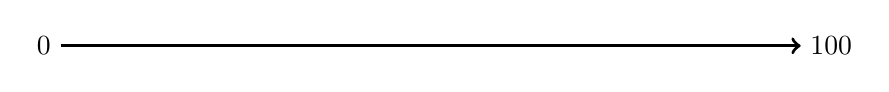
\begin{tikzpicture}
        \node (A) at (0, 0) {0};
        \node (B) at (10, 0) {100};
        \draw [very thick, ->] (A) -- (B);
    \end{tikzpicture}
\end{frame}

\begin{frame}
    \begin{center}
        G\^{e}m \(\frac{2}{3}\)an y cymedr.
    \end{center}
\end{frame}

\begin{frame}
    \begin{center}
        \href{https://www.youtube.com/watch?v=p3Uos2fzIJ0}{Golden Balls}
    \end{center}
\end{frame}

\begin{frame}
    \begin{center}
        \Huge
        \begin{tabular}{|c|c|c|}
            \hline
                   & C        & B        \\
            \hline
            C      & \(2, 2\) & \(5, 0\) \\
            \hline
            B      & \(0, 5\) & \(4, 4\) \\
            \hline
        \end{tabular}
    \end{center}
\end{frame}

\begin{frame}
    \begin{center}
        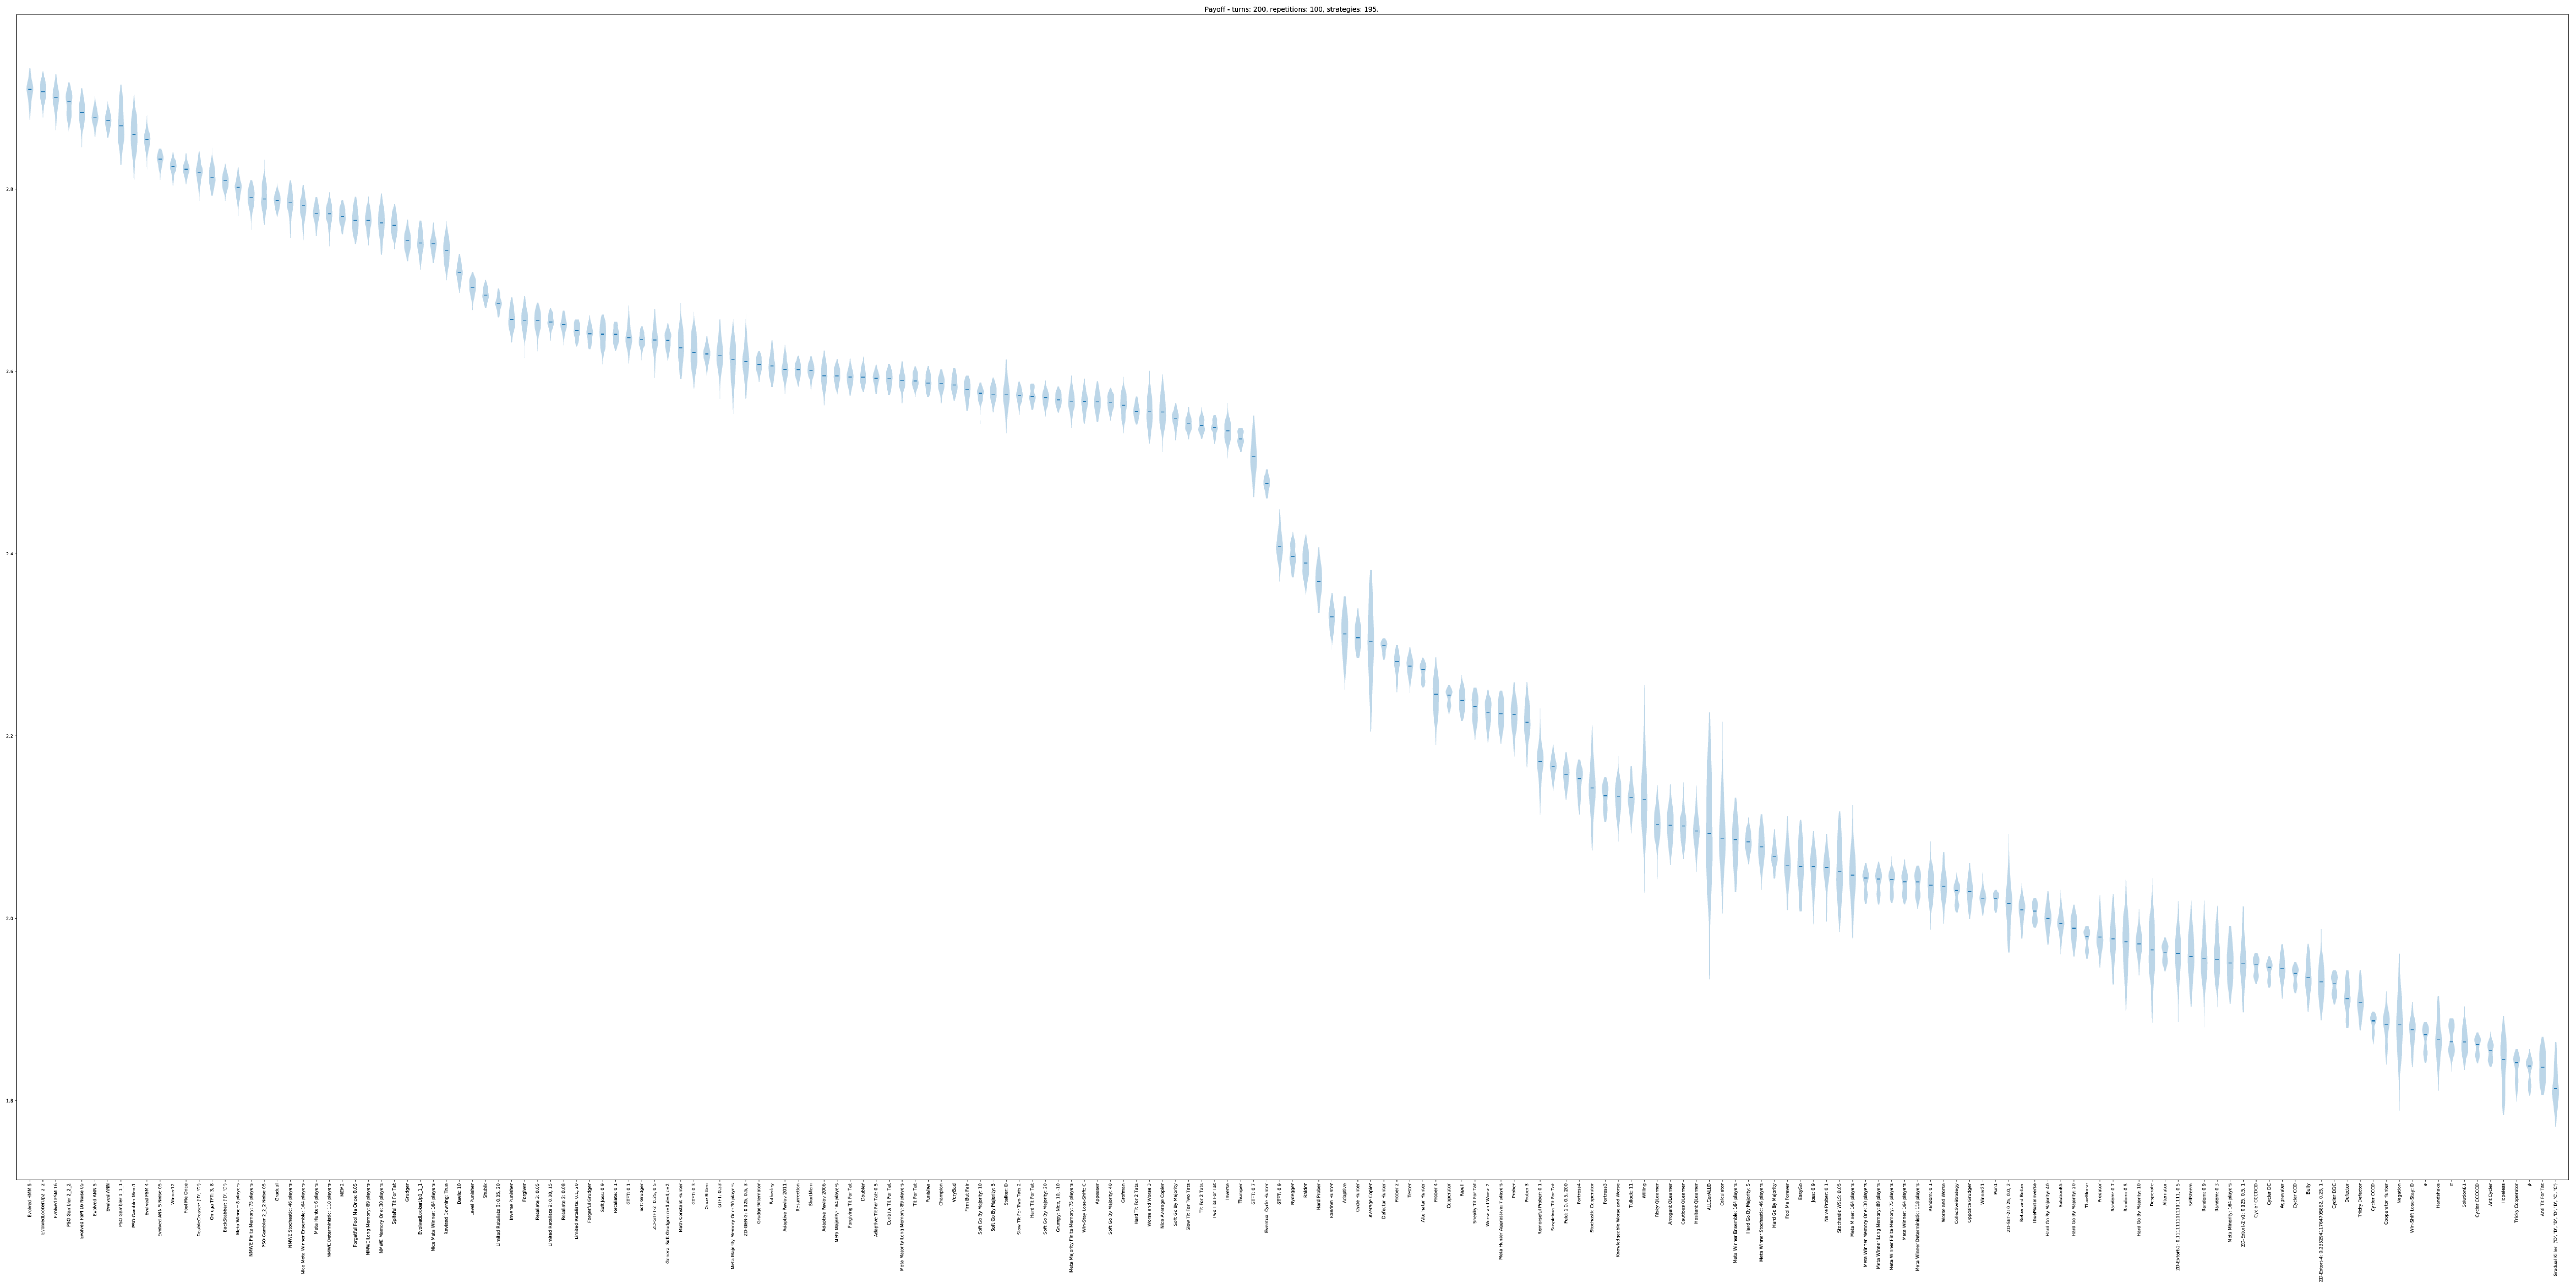
\includegraphics[width=\textwidth]{img/fulltournament.pdf}
    \end{center}
\end{frame}

\end{document}
